\documentclass{article}

\input{../../../latex_preambule_style/preambule}
\input{../../../latex_preambule_style/stylecours}
\input{../../../latex_preambule_style/styleExercices}
\input{../../../latex_preambule_style/bas_de_page_quatrieme}

%%%%%%%%%%%%%%%  Indentation  %%%%%%%%%%%%%%%%%%
\parindent=0pt
%%%%%%%%%%%%%%%%%%%%%%%%%%%%%%%%%%%%%%%%%%%%%%%%
\begin{document}

\begin{titre}[Les statistiques]

{\color{bleu3}{\LARGE Utilisation d'un tableur} \hfill{Niveau 1}}
\end{titre}



\begin{CpsCol}
\textbf{Interpréter, représenter et traiter des données}
\begin{description}
\item[$\square$] Calculer une fréquence
\item[$\square$] Utiliser un tableur pour effectuer des calcul
\end{description}
\end{CpsCol}

\begin{Rec}

Le travail de statistiques est souvent fastidieux, on a toujours recours à un tableur lorsque les données sont trop importantes. Une feuille de calcul d'un tableur se présente comme cela, en cellules. La cellule rouge est la cellule C3.

L'intérêt d'un tableur est le calcul automatique des caractéristiques demandées : moyenne, fréquence, effectif cumulés,... Pour cela, il faut utiliser des formules mathématiques.

\vspace{0.4cm}

\begin{tabular}{|c|m{2cm}|m{2cm}|m{2cm}|m{2cm}|m{2cm}|}
\hline 
\rowcolor{gray} & A & B & C & D &...\\ 
\hline 
\cellcolor{gray}1 & &4 &  & &  \\ 
\hline 
\cellcolor{gray}2 & & & 5 & &   \\ 
\hline 
\cellcolor{gray}3 & & & \cellcolor{red} & &  \\ 
\hline 
\cellcolor{gray}... & & &  & & \\ 
\hline 
\end{tabular} 

\subsubsection*{Quelques formules : Utilisation du signe = avant toute formule}

\begin{description}
\item[=a+b] calcule la somme de  $a$ et de $b$. 
\item[=SOMME(plage)] calcule la somme des cellules dans une plage rectangulaire.
\item[=NB.SI(plage;critère] renvoie parmi les cellules de la plage celle qui vérifie le critères.
\item[=a/b] calcule le quotient de  $a$ par $b$. $b$ doit être non nul.
\end{description}

\subsubsection*{Utilisations}
\begin{description}[leftmargin=*]
\item Pour calculer 4+5 dans la cellule D3, on tapera dans la cellule D3, \textbf{=B1+C2}. Lorsque une des valeurs des cellules B1 ou C2 change, la somme change alors. 
\item Pour calculer 4/5 dans la cellule B3, on tapera dans la cellule DB3, \textbf{=B1/C2}. 
\end{description}

\subsection*{Application concrète}

Voici les notes obtenues à un contrôle sur 10 par une classe de quatrième :\\
0 -- 1 -- 2 -- 2 -- 3 -- 3 -- 3 -- 3 -- 4 -- 4 -- 5 -- 5 -- 5 -- 6 -- 6 -- 6 -- 7 -- 7 -- 8 -- 8 -- 8 -- 9 -- 9 -- 10 -- 10.

\begin{enumerate}
\item Créer un tableau sur une feuille de calcul et complète le tableau ci-dessous avec les formules adéquates.
\item Combien d'élèves ont obtenu moins de 5 ?
\item Quel est le pourcentage d'élèves qui ont obtenu 8 ?
\item Quel est le pourcentage d'élèves qui ont obtenu au moins 8 ?
\item Change un 3 et par un 8 dans la série statistique. Remarque le changement de résultats.
\end{enumerate}

\begin{tabular}{|p{4.2cm}*{11}{|p{5mm}}|p{8mm}|}
\hline
Note&0 & 1 & 2& 3 & 4 & 5 & 6&7 &8 &9 &10&Total \\
\hline
Effectifs&1 & 1 & 2& &&&& & &&& \\
\hline
Effectifs cumulés&1 & 2 & 4& &  & & & && & & \\
\hline
Fréquences &0,04 & 0,04 & 0,08 & &  & & & & & & & \\
\hline
Fréquences cumulées &0,04  & 0,08  & 0,16  &  &  & & & & & & & \\
\hline
\end{tabular}




\subsubsection*{Effectifs -- Effectifs cumulés}
	Pour chaque note, {\em l'effectif} est le nombre d'élèves ayant eu cette note.	Par exemple (dans le tableau), 1 élève a eu 0 ;	2 élèves ont eu 1\dots\\ 
	Pour chaque note, {\em l'effectif cumulé} est le nombre d'élèves ayant eu cette note ou une note inférieure. Pour le calculer, il suffit à chaque fois de cumuler les effectifs.\\
	Par exemple (dans le tableau), 1 élève a eu 0 ;	$1+2=3$ élèves ont eu 1 au plus ; $3+4=7$ élèves ont eu 2 au plus\dots
	
\subsubsection*{Fréquences -- Fréquences cumulées}
	Pour chaque note, {\em la fréquence} exprime la proportion d'élèves. Par exemple, sur les 20 élèves, 4 élèves ont eu une note de 2.
	La proportion est de 4 sur 20 ou $4\over20$ que l'on exprime en \%\ par le calcul $100\times{4\over20}=20$.\\
	Comme pour les effectifs cumulés, les {\em fréquences cumulées}	sont obtenues en cumulant les fréquences.
\end{Rec}

\begin{DefT}{Fréquence}
La population $P$ étudiée a un effectif total égal à $N$.
La fréquence $f$ d'un sous ensemble de la population, appelé $A$, d'effectif $n$ est le quotient de cet effectif sur l'effectif total $N$. On écrit alors $f_A=\frac{n}{N}$.
\end{DefT}


\begin{Ex}
Une classe de Quatrième compte 25 élèves dont 12 filles.\\
La population est l'ensemble des élèves de la classe. L'effectif de la population est égal à 25, c'est l'effectif total : $N=25$.\\
Pour calculer la fréquence des filles dans cette classe, on détermine l'effectif de ce sous ensemble : les filles. $n=12$\\
Donc $f_{filles}=\frac{12}{25}$.
\end{Ex}

\begin{AD}

Lors du concours Algoréa, les 12\% meilleurs élèves sont qualifiés pour le tour suivant. 
\begin{description}
\item[•] En sixième, Mathis est arrivée $682^{ième}$ sur 6800 participants.
\item[•] En cinquième, Pol est arrivé $524^{ième}$ sur 5200 participants.
\item[•] En quatrième, Luisa est arrivée $855^{ième}$ sur 8200 participants.
\item[•] En troisième, Rafaela est arrivée $423^{ième}$ sur 4500 participants.
\end{description}
Quel élèves ont été sélectionnés pour le tour suivant ?

\end{AD}


\begin{AD}

Lors de la première édition de la Course aux Nombres, les 24 élèves de la classe de Cinquième 2 en Colombie ont obtenu les résultats suivants. Les notes sont évaluées sur 30 points.


\begin{enumerate}
\item Reproduire la feuille de calcul comme indiqué ci dessous.

\begin{tabular}{|c|c|c|c|c|c|c|c|c|c|}
\hline 
\rowcolor{gray} & A & B & C & D & E & F & G & H & I \\ 
\hline 
\cellcolor{gray} 1 & 11 & 16 & 22 & 20 & 26 &  &  & Nombres d'élèves total &  \\ 
\hline 
\cellcolor{gray}2& 26 & 18 & 26 & 19& 16 &  &  & Nombre d'élèves dont la nombre est égale à 22 &  \\ 
\hline 
\cellcolor{gray}3 & 17 &27 & 18 & 16 & 22 &  & & Fréquence d'élèves dont la note est égale à 22 &  \\ 
\hline 
\cellcolor{gray}4 & 16 & 19 & 11 & 21 & 17 & &  & Nombre d'élèves dont la note est égale à 19 &  \\ 
\hline 
\cellcolor{gray}5 & 22 & 15 & 22 & 23 &  &  &  & Fréquence d'élèves dont la note est égale à 19 &  \\ 
\hline 
\end{tabular} 

\item  
\begin{enumerate}
\item  Déterminer dans la cellule I1 le nombre d'élèves participants à ce jeu. 
Rappel : Pour déterminer le nombre de cases remplies d'un tableau, on utilise la syntaxe : =NB(A1:E5). 
\item  Déterminer dans la cellule I2 le nombre d'élèves dont la note est égale à 22 ? 
Rappel : Pour déterminer le nombre de cases remplies avec la valeur 22, on utilise la syntaxe : =NB.SI(A1:E5;22). 
\item  Calcule dans la cellule I3 la fréquence des élèves ayant obtenu 22.
\end{enumerate}
\item  
\begin{enumerate}
\item Détermine la moyenne de cette classe. On pourra utiliser la syntaxe "=MOYENNE(A1:E5)".
\item Explique par une phrase le calcul du tableur pour donner la moyenne.
\item 
\begin{enumerate}
\item Complète le tableau ci-dessous.

\begin{tabular}{|c|c|c|c|c|c|c|}
\hline 
Notes & $[0;5[$ &  $[5;10[$  &  $[10;15[$  &  $[15;20[$  &  $[20;25[$  &  $[25;30]$  \\ 
\hline 
Fréquence &  &  &  &  &  &  \\ 
\hline 
\end{tabular} 

\item Calcule la moyenne avec ce regroupement.	
\end{enumerate}
\item Création d'un diagramme avec un tableur
\begin{enumerate}
\item  Sélectionne la plage de données A1:E5 puis clique sur l'icône graphique
\item  Quel est le problème de la plage de données A1:E5 ?
\end{enumerate}

\end{enumerate}
\end{enumerate}




\end{AD}


\begin{autoeval}
\begin{tabular}{p{12cm}p{0.5cm}p{0.5cm}p{0.5cm}p{1cm}}
\textbf{Compétences visées} &  M I & MF & MF  & TBM \vcomp \\ 
Calculer une fréquence & $\square$ & $\square$  & $\square$ & $\square$ \vcomp \\ 
Utiliser un tableur pour effectuer des calcul & $\square$ & $\square$ & $\square$ & $\square$ \vcomp \\ 
\end{tabular}
{\footnotesize MI : maitrise insuffisante ; MF = Maitrise fragile ; MS = Maitrise satisfaisante ; TBM = Très bonne maitrise}
 
\end{autoeval}
\newpage
\begin{titre}[Les statistiques]

{\color{bleu3}{\LARGE Lecture et représentation de données} \hfill{Niveau 2}}
\end{titre}



\begin{CpsCol}
\textbf{Interpréter, représenter et traiter des données}
\begin{description}
\item[$\square$] Lire des données sur différents supports
\end{description}
\end{CpsCol}

\begin{AD}

Les notes d'une classe de Seconde sont représentées par le diagramme à bâtons ci-dessous.

\begin{center}
\definecolor{ffqqqq}{rgb}{1.,0.,0.}
\definecolor{cqcqcq}{rgb}{0.7529411764705882,0.7529411764705882,0.7529411764705882}
\begin{tikzpicture}[line cap=round,line join=round,>=triangle 45,x=1.0cm,y=1.0cm]
\draw [color=cqcqcq,, xstep=1.0cm,ystep=1.0cm] (-0.76,-1.1175) grid (11.64,7.2625);
\draw[->,color=black] (-0.76,0.) -- (11.64,0.);
\foreach \x in {,1.,2.,3.,4.,5.,6.,7.,8.,9.,10.,11.}
\draw[shift={(\x,0)},color=black] (0pt,2pt) -- (0pt,-2pt) node[below] {\footnotesize $\x$};
\draw[->,color=black] (0.,-1.1175) -- (0.,7.2625);
\foreach \y in {-1.,1.,2.,3.,4.,5.,6.,7.}
\draw[shift={(0,\y)},color=black] (2pt,0pt) -- (-2pt,0pt) node[left] {\footnotesize $\y$};
\draw[color=black] (0pt,-10pt) node[right] {\footnotesize $0$};
\clip(-0.76,-1.1175) rectangle (11.64,7.2625);
\draw [line width=2.pt,color=ffqqqq] (1.,0.)-- (1.,2.);
\draw [line width=1.2pt,color=ffqqqq] (2.,0.)-- (2.,3.);
\draw [line width=1.2pt,color=ffqqqq] (3.,0.)-- (3.,2.);
\draw [line width=1.2pt,color=ffqqqq] (4.,0.)-- (4.,4.);
\draw [line width=1.2pt,color=ffqqqq] (5.,0.)-- (5.,6.);
\draw [line width=1.2pt,color=ffqqqq] (6.,0.)-- (6.,5.);
\draw [line width=1.2pt,color=ffqqqq] (7.,0.)-- (7.,5.);
\draw [line width=1.2pt,color=ffqqqq] (8.,0.)-- (8.,4.);
\draw [line width=1.2pt,color=ffqqqq] (9.,0.)-- (9.,2.);
\draw [line width=1.2pt,color=ffqqqq] (10.,0.)-- (10.,1.);
\draw (10.08,-0.4975) node[anchor=north west] {note sur 10};
\draw (0.12,6.5425) node[anchor=north west] {Effectif};
\end{tikzpicture}
\end{center}

\begin{enumerate}
\item Quelle est la note plus plus souvent obtenue ? Cette valeur s'appelle \textbf{le mode}.
\item Combien d'élèves composent cette classe ?
\end{enumerate}

\end{AD}

\begin{AD}

Évolution de la population chinoise

\begin{center}
\begin{tabular}{|c|c|c|}
\hline 
\rowcolor{bleu1!25!white} & 1950 & 2009  \\ 
\hline 
\cellcolor{bleu1!25!white}  Nombre d'habitants &  \np{554760} millions & 1,3 milliards  \\ 
\hline 
\cellcolor{bleu1!25!white} Espérance de vie & 39 & 73 \\ 
\hline 
\cellcolor{bleu1!25!white}IDH ( indicateur de développement humain) & 0,55 (1980) & 0,772 \\ 
\hline 
\cellcolor{bleu1!25!white}Part de personnes sachant lire et écrire (en \%) & H : 79\% et F :54,4\% &  H :94,1\% et F :82,1\%  \\ 
\hline 
\cellcolor{bleu1!25!white}Mortalité infantile (pour 1000 naissances) & 195 & Garçons(17), Filles(24) \\ 
\hline 
\cellcolor{bleu1!25!white}Fécondité & 6,6 & 1,7 \\ 
\hline 
\end{tabular} 
\end{center}

\begin{enumerate}
\item Quelle est l'évolution du nombre d'habitants en Chine entre  1950 et 2009 ?
\item Combien de femmes savent lire en 1950 ? en 2009 ? 
\item Quelle est l'évolution de l'espérance de vie en Chine entre 1950 et 2009 ?
\item Dans un village de \np{1280} habitants comprenant 45\% d'hommes, combien d'habitants savent lire ?
\end{enumerate}


\end{AD}


\begin{AD}

\begin{minipage}{0.5\linewidth}
Le graphique ci-dessous montre les résultats à un contrôle de sciences obtenus par deux groupes d'élèves, désignés par « Groupe A » et « Groupe B ». 
La note moyenne pour le Groupe A est de 62,0 et de 64,5 pour le Groupe B. Les élèves réussissent ce contrôle lorsque leur note est de 50 points ou davantage. Sur la base de ce graphique, le professeur conclut que le Groupe B a mieux réussi ce contrôle que le Groupe A. Les élèves du Groupe A ne sont pas d'accord avec le professeur. Ils essaient de le convaincre que le Groupe B n'a pas nécessairement mieux réussi. \hfill{{\scriptsize D'après PISA 2009}}
\end{minipage}
\begin{minipage}{0.5\linewidth}
\begin{center}
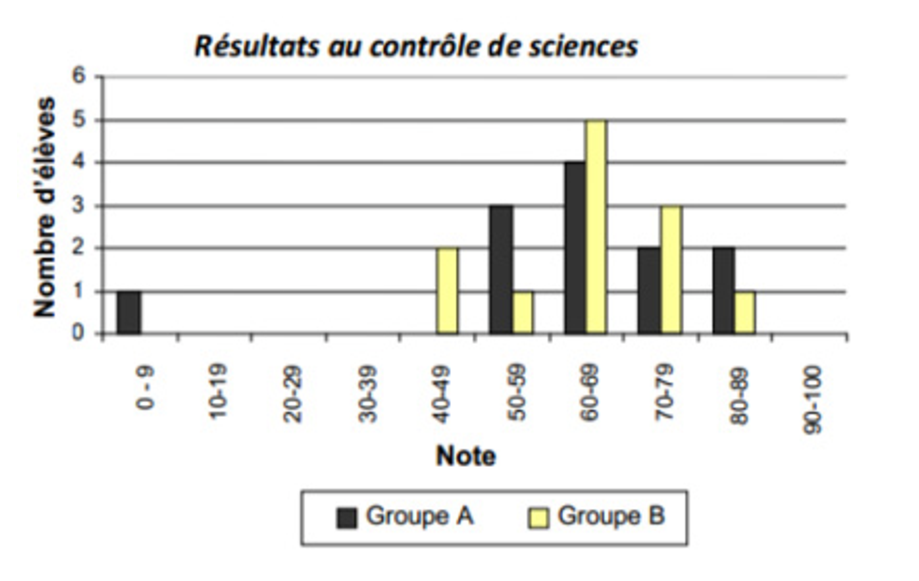
\includegraphics[scale=0.6]{Stat-13.eps} 
\end{center}
\end{minipage}
En vous servant du graphique, donnez un argument mathématique que les élèves du Groupe A pourraient utiliser. 


\end{AD}

\begin{AD}

On a représenté sur le diagramme suivant les vols du mois de février d’une compagnie aérienne.  
\begin{center}
\definecolor{xdxdff}{rgb}{0.49019607843137253,0.49019607843137253,1.}
\definecolor{ffdxqq}{rgb}{1.,0.8431372549019608,0.}
\definecolor{ffffqq}{rgb}{1.,1.,0.}
\definecolor{ffxfqq}{rgb}{1.,0.4980392156862745,0.}
\definecolor{ffqqqq}{rgb}{1.,0.,0.}
\definecolor{xfqqff}{rgb}{0.4980392156862745,0.,1.}
\definecolor{qqqqff}{rgb}{0.,0.,1.}
\begin{tikzpicture}[line cap=round,line join=round,>=triangle 45,x=1.0cm,y=1.0cm]
\clip(-0.096,-0.204) rectangle (18.304,8.336);
\draw[color=xfqqff,fill=xfqqff,fill opacity=1.0] (5.,3.5757359312880714) -- (5.424264068711929,3.5757359312880714) -- (5.424264068711929,4.) -- (5.,4.) -- cycle; 
\draw [shift={(5.,4.)},color=ffqqqq,fill=ffqqqq,fill opacity=1.0] (0,0) -- (0.:0.6) arc (0.:30.488940499830935:0.6) -- cycle;
\draw [shift={(5.,4.)},color=ffxfqq,fill=ffxfqq,fill opacity=0.95] (0,0) -- (30.488940499830935:0.6) arc (30.488940499830935:59.44286434307001:0.6) -- cycle;
\draw [shift={(5.,4.)},fill=black,fill opacity=1.0] (0,0) -- (59.44286434307001:0.6) arc (59.44286434307001:90.:0.6) -- cycle;
\draw [shift={(5.,4.)},color=qqqqff,fill=qqqqff,fill opacity=0.44]  plot[domain=1.5707963267948966:4.71238898038469,variable=\t]({1.*4.*cos(\t r)+0.*4.*sin(\t r)},{0.*4.*cos(\t r)+1.*4.*sin(\t r)});
\draw [shift={(5.,4.)},color=xfqqff,fill=xfqqff,fill opacity=0.66]  (0,0) --  plot[domain=-1.5707963267948966:0.,variable=\t]({1.*4.*cos(\t r)+0.*4.*sin(\t r)},{0.*4.*cos(\t r)+1.*4.*sin(\t r)}) -- cycle ;
\draw [shift={(5.,4.)},color=ffqqqq,fill=ffqqqq,fill opacity=0.6]  (0,0) --  plot[domain=0.:0.5321323971666955,variable=\t]({1.*4.*cos(\t r)+0.*4.*sin(\t r)},{0.*4.*cos(\t r)+1.*4.*sin(\t r)}) -- cycle ;
\draw [shift={(5.,4.)},color=ffxfqq,fill=ffxfqq,fill opacity=0.4]  (0,0) --  plot[domain=0.5321323971666955:1.037473699602908,variable=\t]({1.*3.973415659102379*cos(\t r)+0.*3.973415659102379*sin(\t r)},{0.*3.973415659102379*cos(\t r)+1.*3.973415659102379*sin(\t r)}) -- cycle ;
\draw [shift={(5.,4.)},color=ffffqq,fill=ffffqq,fill opacity=0.5]  (0,0) --  plot[domain=1.037473699602908:1.5707963267948966,variable=\t]({1.*4.*cos(\t r)+0.*4.*sin(\t r)},{0.*4.*cos(\t r)+1.*4.*sin(\t r)}) -- cycle ;
\draw (10.644,6.776) node[anchor=north west] {Vols vers l'Asie};
\draw (10.664,6.176) node[anchor=north west] {Vols vers l'Afrique};
\draw (10.664,5.616) node[anchor=north west] {Vols vers l'Amérique};
\draw (10.704,5.056) node[anchor=north west] {Vols vers l'Europe};
\draw (10.724,4.436) node[anchor=north west] {Vols vers la France};
\begin{scriptsize}
\draw [fill=ffffqq] (10.304,6.636) circle (2.5pt);
\draw [fill=ffdxqq] (10.304,6.036) circle (2.5pt);
\draw [fill=ffqqqq] (10.324,5.436) circle (2.5pt);
\draw [fill=xfqqff] (10.344,4.836) circle (2.5pt);
\draw [fill=xdxdff] (10.364,4.236) circle (2.5pt);
\end{scriptsize}
\end{tikzpicture}
\end{center}

\begin{minipage}{8cm}
Dans chaque cas, quelle fréquence représentent les vols vers la France, l’Europe et l’Asie. 
\end{minipage}
\begin{minipage}{1cm}
$~~$
\end{minipage}
\begin{minipage}{8cm}
Au mois de février, cette compagnie a affrété 576 vols. Calculer le nombre de vols vers la France, l’Europe et l’Asie. 
\end{minipage}

\end{AD}



\begin{autoeval}
\begin{tabular}{p{12cm}p{0.5cm}p{0.5cm}p{0.5cm}p{1cm}}
\textbf{Compétences visées} &  M I & MF & MF  & TBM \vcomp \\ 
Lire des données sur différents supports & $\square$ & $\square$  & $\square$ & $\square$ \vcomp \\ 
\end{tabular}
{\footnotesize MI : maitrise insuffisante ; MF = Maitrise fragile ; MS = Maitrise satisfaisante ; TBM = Très bonne maitrise}
 
\end{autoeval} % Représenter des données, calcul de fréquence
\newpage
\begin{titre}[Les statistiques]

{\color{bleu3}{\LARGE Calcul de moyenne} \hfill{Niveau 2}}
\end{titre}



\begin{CpsCol}
\textbf{Interpréter, représenter et traiter des données}
\begin{description}
\item[$\square$] Calculer une moyenne
\item[$\square$] Interpréter une caractéristique de position
\end{description}
\end{CpsCol}

\begin{Rec}

Si 2/5 des habitants d'un pays ont au moins 50 ans et 1/3 des habitants de ce pays ont moins de 20 ans, est-il possible que l'âge moyen de la population soit de 40 ans ?

\hfill{D’après le cadre d’évaluation «PISA 2006»:}
 
\hfill{items libérés Mathématiques OCDE/DEPP – janvier 2011}


\end{Rec}

\begin{DefT}{moyenne}
La \textbf{moyenne} d'une série statistique est le quotient de la somme de TOUTES les valeurs par l'effectif total de cette série.
\end{DefT}

\begin{Ex}
Voici les notes obtenues par Aurélie en Mathématiques au cours de l'année. 
\begin{itemize}
\item	1er trimestre :		10 – 9 – 11 – 12 – 11,5 – 14 – 12
\item	2ème trimestre :	9,5 – 11 – 12,5 – 8 – 13 – 18
\item	3ème trimestre :	8 – 9 – 14 – 12 – 10 – 13 – 11,5
\end{itemize}
Calculons sa moyenne annuelle :
		$m1 =\frac{10+9+11+\ldots{}+11,5}{20}=\frac{229}{20}=11,45$ 
\end{Ex}
		

\begin{AD}

\begin{multicols}{2}
Voici ci-contre la répartition par âge des membres d'un club d'échec.
Quel est l'age moyen des adhérents ?

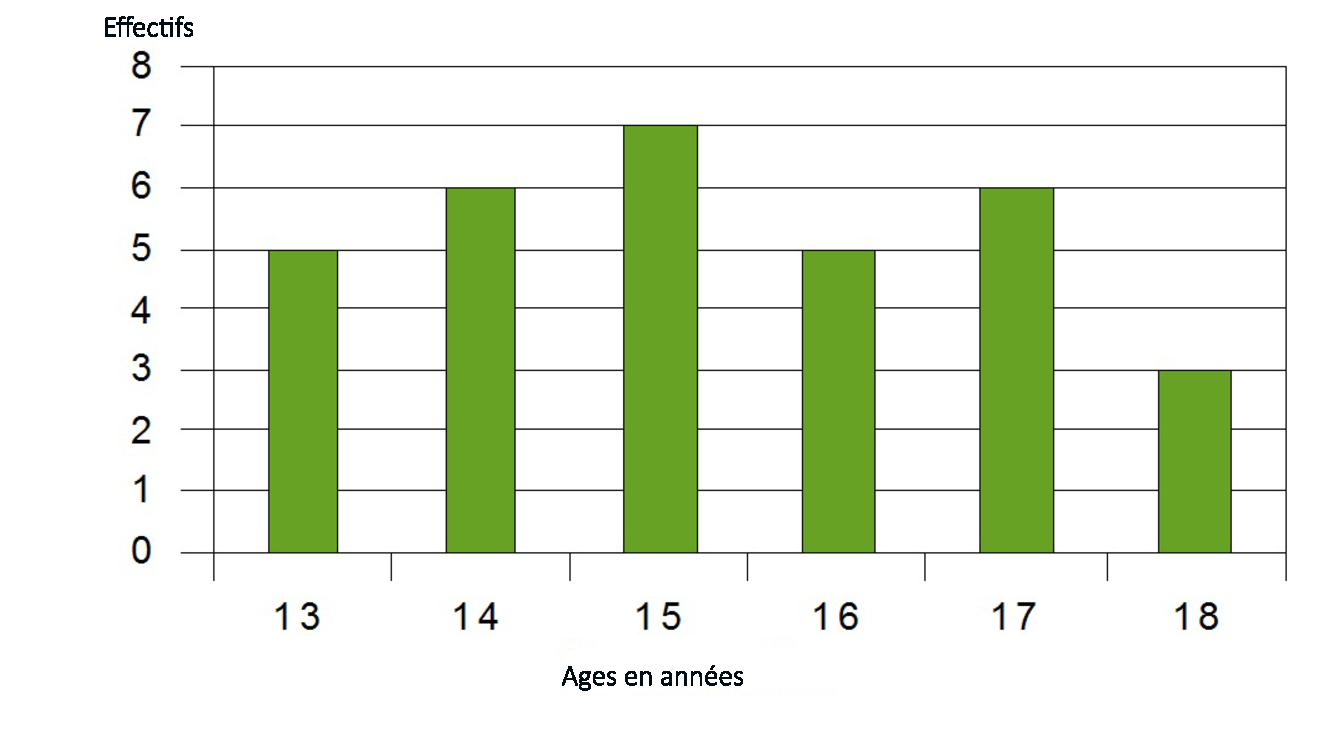
\includegraphics[scale=0.35]{Stat-cours1.eps} 
\end{multicols}	
\end{AD}


 


\begin{tabular}{|c|c|c|c|c|c|}
\hline 
heures & $0\leq h < 4$ & $4 \leq h < 8$ & $8 \leq h < 12$ & $12 \leq h < 16$ & $16 \leq h$ \\ 
\hline 
températures & 12 & 18 & 22 & 30 & 26 \\ 
\hline 
\end{tabular} 



\subsection*{Moyenne de moyennes}
\begin{Ex}
		
Avec l'exemple précédent :
\begin{itemize}
\item 		1er trimestre :	  la moyenne d'Aurélie est $11,36$ ;
\item		2ème trimestre : la moyenne d'Aurélie est $12$ ;
\item		3ème trimestre : la moyenne d'Aurélie est $11,07$.
\end{itemize}
Calculons la moyenne de ses moyennes trimestrielles :
		$m2 =\frac{11,36+12+11,07}{3}=\frac{34,43}{3}$ donc  		$m2\approx 11,48$
\end{Ex}
				
		
		
\begin{Rq}	
Cette moyenne est rarement égale à la moyenne de la série.

La moyenne est toujours comprise entre la plus petite valeur et la plus grande valeur de la série statistique.
\end{Rq}



\begin{AD}

Voici les notes d'un élève de 4\ieme\ en mathématiques.
\medskip
\begin{description}
 \item [1\ier\ trimestre] 15\kern5mm 10\kern5mm 8\kern5mm 13\kern5mm 10
\item[2\ieme\ trimestre] 13\kern5mm 9\kern5mm 7\kern5mm 14\kern5mm 13\kern5mm 16
\item[3\ieme\ trimestre] 12\kern5mm 15\kern5mm 17\kern5mm 14\kern5mm 12
\end{description}
\begin{enumerate}
  \item Calcule sa moyenne pour chacun des trois trimestres.
  \item Calcule la moyenne des moyennes des trois trimestres.
  \item Calcule la moyenne de l'ensemble de ses notes sur son année de 4\ieme.\\Que remarque-t-on ?
\end{enumerate}
\end{AD}

\begin{AD}

On a trié 4 paquets de 40 M\&M's et on a obtenu les résultats suivants : 


\begin{center}
 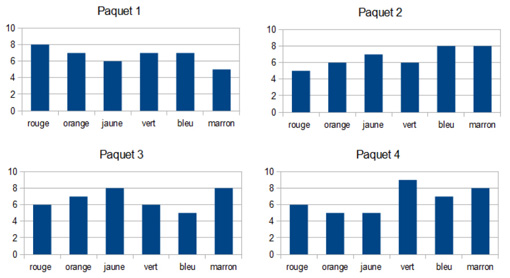
\includegraphics[scale=0.5]{mms1.jpg}
 \end{center} 


\begin{enumerate}
\item Calcule le nombre de bonbons bleus dans ces 4 paquets.
\item Combien en moyenne a-t-on de M\&M's bleus par paquets ? 
\end{enumerate}


\end{AD}

\begin{Exo}

\begin{minipage}[top]{10cm}
L'entreprise est à la recherche de qualifications de plus en plus élevées pour faire face au développement de technologies en constante évolution et pour une bonne compréhension des consignes de travail. Lors de sa scolarité, un jeune doit développer de l'intérêt et de la curiosité, si utiles pour réussir ensuite sa vie professionnelle. Face au nombre, en baisse mais encore inquiétant, de sorties du système scolaire sans qualification, il paraît intéressant d'étudier ce phénomène du point de vue européen à la lumière des mathématiques. En France, 13\% des jeunes de 18 à 24 ans qui ne poursuivent pas d'études ni de formation n'ont ni CAP, ni BEP, ni bac et sont sortants précoces.
\end{minipage}
\begin{minipage}{6cm}
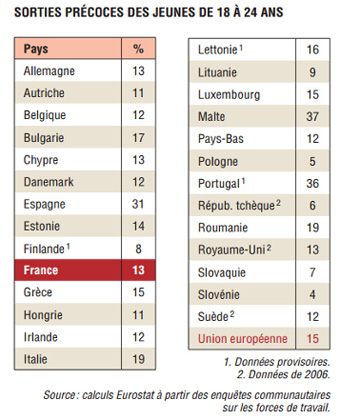
\includegraphics[scale=0.5]{stat12.jpg} 
\end{minipage}

\begin{enumerate}
\item Calculer la moyenne des sorties précoces en Europe à l'aide des données du tableau. Que remarquez-vous ? Justifier.
\item Tracer une représentation graphique de ce tableau sur tableur ou sur une feuille.
\item Compléter le tableau suivant et construire l'histogramme de cette série.

\begin{tabular}{|c|c|c|c|c|c|c|}
\hline 
Sorties précoces en 2007 & [0;5[ & [5;10[ & [10;15[ & [15;20[ & [20;25[ & [25;30] \\ 
\hline 
Nombre de pays européens &  &  &  &  &  &  \\ 
\hline 
\end{tabular} 

\item Calculer la moyenne des sorties précoces en Europe à l'aide de la question 3. Comparer le résultat avec la question 1.  
\end{enumerate}




  
\end{Exo}



\begin{DefT}{moyenne pondérée}
La \textbf{moyenne pondérée} d’une série statistique est le quotient de la somme
de TOUTES les valeurs multipliées chacune par leur coefficients
par la somme de ces coefficients.
\end{DefT}

\begin{AD}

Pierre, Jean et Alain ont passé un examen comportant quatre
disciplines. Pour être reçu, il faut atteindre 10 de moyenne.
\begin{enumerate}
\item Calculer la moyenne, sans coefficient, des trois candidats.
\begin{center}
  \begin{tabular}{|c|c|c|c|c|}
\cline{2-5}
\multicolumn{1}{c|}{}&Français&Mathématiques&Anglais&Technologie\\
\hline
Pierre&15&9&11&7\\
\hline
Jean&10&11&12&9\\
\hline
Alain&7&14&13&8\\
\hline
  \end{tabular}
\end{center}
\item Pour cet examen, le français, les mathématiques, l'anglais et la
technologie ont respectivement pour coefficient 6; 4; 2 et 5.\par
Calculer la moyenne pondérée de chaque candidat et dire s'ils sont reçus
ou non.
\end{enumerate}
\end{AD}

\begin{AD}

Lors d'un test d'endurance, plusieurs élèves ont eu 12 minutes pour
parcourir la plus grande distance possible. Voici les résultats des
élèves :
2230 -- 2450 -- 1890 -- 1850 -- 2650 -- 2630 -- 2110 -- 2250 -- 2180 --
1980 -- 2000 -- 2850 -- 1950 -- 2920 -- 1975 -- 1910 -- 1860 -- 1930 --
2010 -- 2400 -- 2650 -- 2320 -- 2190 -- 2730 -- 2120 -- 2380 -- 2220.

\begin{enumerate}
\item
Calcule la moyenne des distances parcourues.

\item
On veut calculer la moyenne approximative des distances parcourues.
Pour cela, dénombrer le nombre d'élèves dans chacun des intervalles
suivants :\\
\hskip 0pt plus 500pt minus 500pt\begin{tabular}{|*{6}{c|}}
\hline
$[1800 ; 2000 [$ & $[2000 ; 2200 [$ &
$[2200 ; 2400 [$ & $[2400 ; 2600 [$ &
$[2600 ; 2800 [$ & $[2800 ; 3000 [$ \\
\hline
&&
 &&& \\
\hline
\end{tabular}\hskip 0pt plus 500 pt minus 500 pt\strut
\item
Calculer une moyenne approchée en remplaçant la distance de chaque élève
	par le début de chaque intervalle (1800 pour le premier, 2000 pour
	le deuxième,\dots) en pensant à remplacer chaque série de nombres
	identiques par une multiplication.
	
\item Reprendre la question précédente en 
	remplaçant la distance de chaque élève
	par le milieu de chaque intervalle (1900 pour le premier, 2100 pour
	le deuxième,\dots)
	
\item Reprendre la question précédente en 
	remplaçant la distance de chaque élève
	par la fin de chaque intervalle (2000 pour le premier, 2200 pour
	le deuxième,\dots)
	
\end{enumerate}
\end{AD}

\begin{AD}

Le professeur d'EPS a relevé les performances ci-dessous :
\begin{center}
  \begin{tabularx}{0.85\linewidth}{|l|X|X|l|X|X|}
    \hline
\multicolumn{1}{|c|}{Noms}&Temps au 80~m (s)&Hauteur du saut (cm)&\multicolumn{1}{c|}{Noms}&Temps au 80~m (s)&Hauteur du saut (cm)\\
\hline
Charles&\multicolumn{1}{c|}{13}&\multicolumn{1}{c|}{110}&Gérald&\multicolumn{1}{c|}{13,6}&\multicolumn{1}{c|}{115}\\
Bruno&\multicolumn{1}{c|}{12,5}&\multicolumn{1}{c|}{120}&Nicolas&\multicolumn{1}{c|}{13,9}&\multicolumn{1}{c|}{110}\\
Sylvie&\multicolumn{1}{c|}{15}&\multicolumn{1}{c|}{100}&Florence&\multicolumn{1}{c|}{14,7}&\multicolumn{1}{c|}{110}\\
Brice&\multicolumn{1}{c|}{13,2}&\multicolumn{1}{c|}{125}&Daniel&\multicolumn{1}{c|}{13}&\multicolumn{1}{c|}{125}\\
Carine&\multicolumn{1}{c|}{15,4}&\multicolumn{1}{c|}{100}&Viviane&\multicolumn{1}{c|}{16}&\multicolumn{1}{c|}{95}\\
Léon&\multicolumn{1}{c|}{12}&\multicolumn{1}{c|}{135}&Barbara&\multicolumn{1}{c|}{15,1}&\multicolumn{1}{c|}{105}\\
Christian&\multicolumn{1}{c|}{12,6}&\multicolumn{1}{c|}{130}&Jeanne&\multicolumn{1}{c|}{14,9}&\multicolumn{1}{c|}{110}\\
\'Elisabeth&\multicolumn{1}{c|}{15,4}&\multicolumn{1}{c|}{95}&Lucie&\multicolumn{1}{c|}{15,4}&\multicolumn{1}{c|}{100}\\
Aude&\multicolumn{1}{c|}{14,9}&\multicolumn{1}{c|}{110}&Odile&\multicolumn{1}{c|}{14,2}&\multicolumn{1}{c|}{85}\\
Cécile&\multicolumn{1}{c|}{16,2}&\multicolumn{1}{c|}{85}&Alice&\multicolumn{1}{c|}{15,6}&\multicolumn{1}{c|}{105}\\
Clément&\multicolumn{1}{c|}{12}&\multicolumn{1}{c|}{140}&Gaël&\multicolumn{1}{c|}{13,5}&\multicolumn{1}{c|}{125}\\
Cathy&\multicolumn{1}{c|}{15,8}&\multicolumn{1}{c|}{100}&Pierre&\multicolumn{1}{c|}{12,3}&\multicolumn{1}{c|}{135}\\
Delphine&\multicolumn{1}{c|}{15}&\multicolumn{1}{c|}{105}&Armand&\multicolumn{1}{c|}{12,8}&\multicolumn{1}{c|}{130}\\
Jacques&\multicolumn{1}{c|}{13,1}&\multicolumn{1}{c|}{135}&Jean&\multicolumn{1}{c|}{13,1}&\multicolumn{1}{c|}{115}\\
André&\multicolumn{1}{c|}{13,9}&\multicolumn{1}{c|}{120}&David&\multicolumn{1}{c|}{12,5}&\multicolumn{1}{c|}{135}\\
\hline
  \end{tabularx}
\end{center}
\begin{enumerate}
  \item
    \begin{enumerate}
    \item Quel est le temps moyen mis pour effectuer le 80~m ?
    \item Combien d'élèves ont un temps supérieur au temps moyen ?
    \end{enumerate}
  \item
    \begin{enumerate}
    \item Quelle est la hauteur moyenne d'un saut ?
    \item Combien d'élèves ont une hauteur inférieure à la hauteur
      moyenne ?
    \end{enumerate}
\end{enumerate}

\end{AD}

\subsection*{Utilisation d'un tableur pour le calcul de la moyenne}

Le tableur est un outil performant pour calculer la moyenne.


\begin{Ex}
Sur la feuille de classeur ci-dessous,
on a calculé la longueur moyenne des prénoms des 684 élèves du collège.\\
		Les longueurs des prénoms sont rangées de la cellule C4 à la cellule C687.\\
		Ces cellules se suivent, on dit qu'elles sont contiguës.\\
		Dans la formule, on utilise alors le symbole \og  deux – points \fg{}.\\
		Dans la zone de saisie des fonctions, on a tapé : =MOYENNE(C4:C687).\\
		
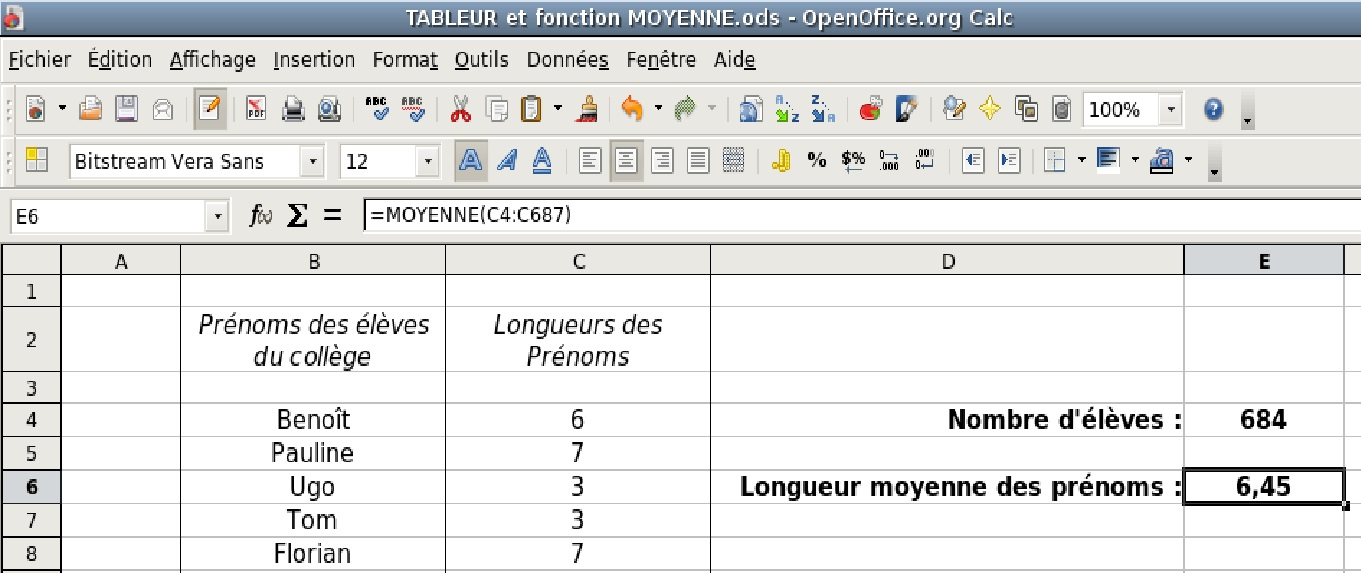
\includegraphics[scale=0.5]{Stat-cours2.jpg} 		
\end{Ex}

\begin{AD}

Lors de la première édition de la Course aux Nombres, les 24 élèves de la classe de Cinquième 2 en Colombie ont obtenu les résultats suivants. Les notes sont évaluées sur 30 points.


\begin{enumerate}
\item Reproduire la feuille de calcul comme indiqué ci dessous.

\begin{tabular}{|c|c|c|c|c|c|c|c|c|c|}
\hline 
\rowcolor{gray} & A & B & C & D & E & F & G & H & I \\ 
\hline 
\cellcolor{gray} 1 & 11 & 16 & 22 & 20 & 26 &  &  & Nombres d'élèves total &  \\ 
\hline 
\cellcolor{gray}2& 26 & 18 & 26 & 19& 16 &  &  & Nombre d'élèves dont la nombre est égale à 22 &  \\ 
\hline 
\cellcolor{gray}3 & 17 &27 & 18 & 16 & 22 &  & & Fréquence d'élèves dont la note est égale à 22 &  \\ 
\hline 
\cellcolor{gray}4 & 16 & 19 & 11 & 21 & 17 & &  & Nombre d'élèves dont la note est égale à 19 &  \\ 
\hline 
\cellcolor{gray}5 & 22 & 15 & 22 & 23 &  &  &  & Fréquence d'élèves dont la note est égale à 19 &  \\ 
\hline 
\end{tabular} 

\item  
\begin{enumerate}
\item  Déterminer dans la cellule I1 le nombre d'élèves participants à ce jeu. 
Rappel : Pour déterminer le nombre de cases remplies d'un tableau, on utilise la syntaxe : =NB(A1:E5). 
\item  Déterminer dans la cellule I2 le nombre d'élèves dont la note est égale à 22 ? 
Rappel : Pour déterminer le nombre de cases remplies avec la valeur 22, on utilise la syntaxe : =NB.SI(A1:E5;22). 
\item  Calcule dans la cellule I3 la fréquence des élèves ayant obtenu 22.
\end{enumerate}
\item  
\begin{enumerate}
\item Détermine la moyenne de cette classe. On pourra utiliser la syntaxe "=MOYENNE(A1:E5)".
\item Explique par une phrase le calcul du tableur pour donner la moyenne.
\item 
\begin{enumerate}
\item Complète le tableau ci-dessous.

\begin{tabular}{|c|c|c|c|c|c|c|}
\hline 
Notes & $[0;5[$ &  $[5;10[$  &  $[10;15[$  &  $[15;20[$  &  $[20;25[$  &  $[25;30]$  \\ 
\hline 
Fréquence &  &  &  &  &  &  \\ 
\hline 
\end{tabular} 

\item Calcule la moyenne avec ce regroupement.	
\end{enumerate}
\item Création d'un diagramme avec un tableur
\begin{enumerate}
\item  Sélectionne la plage de données A1:E5 puis clique sur l'icône graphique
\item  Quel est le problème de la plage de données A1:E5 ?
\end{enumerate}

\end{enumerate}
\end{enumerate}




\end{AD}



\begin{AD}

\begin{enumerate}
\item Explique le fonctionnement de cet algorithme :

\begin{tabular}{|p{10cm}|}
\hline 
\#1. Somme = 0 \\ 
\#2. Moyenne = 0\\ 
\#3. Répéter 4 fois\\ 
\#4. \hspace{1cm} Demander\_une\_valeur x et attendre\\ 
\#5. \hspace{1cm} Lire réponse\\ 
\#6. \hspace{1cm} Somme prend\_la\_valeur Somme +  réponse\\ 
\#7. Moyenne = Somme / 4\\ 
\#8. Afficher Moyenne\\ 
\hline 
\end{tabular} 

\item A l'aide du logiciel Scratch, traduis cet algorithme en programme. 

\end{enumerate}

\end{AD}


\begin{autotest}
\begin{enumerate}
\item On donne les nombres suivants : $$4~~ - ~~ 16 ~~  - ~~ 8 ~~ - ~~ 13 ~~ - ~~ 15 $$
La moyenne est $$a. 11~~ ~~ ~~ b. 11,5 ~~  ~~ ~~ c. 11,2 ~~ ~~ ~~ d. 12$$

\item Pour calculer la moyenne des cellules A5 à B5, avec un tableur, on tape la formule
$$a. MOYENNE(A5:B5)~~ ~~ ~~ b. =MOYENNE(A5:B5) ~~  ~~ ~~ c. MOYENNE(A5;B5) ~~ ~~ ~~ d. =MOYENNE(A5;B5)$$

\item Voici le diagramme à bâtons des notes d'un devoir. 

\definecolor{qqqqff}{rgb}{0.,0.,1.}
\definecolor{cqcqcq}{rgb}{0.7529411764705882,0.7529411764705882,0.7529411764705882}
\begin{tikzpicture}[line cap=round,line join=round,>=triangle 45,x=1.0cm,y=1.0cm]
\draw [color=cqcqcq,, xstep=1.0cm,ystep=1.0cm] (-0.72,-1.1) grid (10.62,7.46);
\draw[->,color=black] (-0.72,0.) -- (10.62,0.);
\foreach \x in {,1.,2.,3.,4.,5.,6.,7.,8.,9.,10.}
\draw[shift={(\x,0)},color=black] (0pt,2pt) -- (0pt,-2pt) node[below] {\footnotesize $\x$};
\draw[->,color=black] (0.,-1.1) -- (0.,7.46);
\foreach \y in {-1.,1.,2.,3.,4.,5.,6.,7.}
\draw[shift={(0,\y)},color=black] (2pt,0pt) -- (-2pt,0pt) node[left] {\footnotesize $\y$};
\draw[color=black] (0pt,-10pt) node[right] {\footnotesize $0$};
\clip(-0.72,-1.1) rectangle (10.62,7.46);
\draw [color=qqqqff] (1.,0.)-- (1.,1.);
\draw [color=qqqqff] (3.,0.)-- (3.,2.);
\draw [color=qqqqff] (4.,0.)-- (4.,3.);
\draw [color=qqqqff] (5.,4.)-- (5.02,-0.14);
\draw [color=qqqqff] (6.,0.)-- (6.,6.);
\draw [color=qqqqff] (7.,6.)-- (7.,0.);
\draw [color=qqqqff] (8.,4.)-- (8.,0.);
\draw [color=qqqqff] (10.,1.)-- (10.,0.);
\draw (9.44,-0.5) node[anchor=north west] {notes};
\draw (0.16,6.42) node[anchor=north west] {Effectifs};
\end{tikzpicture}

La moyenne est $$a. \approx 5,9 ~~ ~~ ~~ b. \approx 6,5 ~~  ~~ ~~ c. \approx 1,7 ~~ ~~ ~~ d. \approx 5,5$$

\item Pierre n'a retrouvé que 7 contrôles où il a obtenu chaque fois 8 sur 10. Il a perdu une copie mais il sait que sa moyenne est de 7,75. Quelle est la note de la copie perdue ?

\item Grégory espère obtenir au Bac 17/20 en Maths, 14/20 en Lettres et 17/20 en Langues. Le coefficient de l'épreuve des maths est 7, celui de l'épreuve des lettres est 3 et celui de l'épreuve des langues est 2. Peut il espérer obtenir la mention "Très bien" ?

\item Le tableau donne le nombre de voitures qui passent dans un virage dangereux où la vitesse est limitée à 60 km/h. 

\begin{tabular}{|c|c|c|c|c|}
\hline 
Vitesse & [30;40[ & [40;50[ & [50;60[ & [60;70[ \\ 
\hline 
Effectif & 15 & 60 & 80 & 25 \\ 
\hline 
\end{tabular} 

Peut on dire les conducteurs respectent la limitation de vitesse ?

\end{enumerate}
\end{autotest}



\begin{autoeval}
\begin{tabular}{p{12cm}p{0.5cm}p{0.5cm}p{0.5cm}p{1cm}}
\textbf{Compétences visées} &  M I & MF & MF  & TBM \vcomp \\ 
Calculer une moyenne & $\square$ & $\square$  & $\square$ & $\square$ \vcomp \\ 
Interpréter une caractéristique de position & $\square$ & $\square$ & $\square$ & $\square$ \vcomp \\ 
\end{tabular}
{\footnotesize MI : maitrise insuffisante ; MF = Maitrise fragile ; MS = Maitrise satisfaisante ; TBM = Très bonne maitrise}
 
\end{autoeval} % Calculer une moyenne à partir de données
\newpage
\begin{titre}[Les statistiques]

{\color{bleu3}{\LARGE Calcul de médiane, d'étendue} \hfill{Niveau 3}}
\end{titre}


\begin{CpsCol}
\textbf{Interpréter, représenter et traiter des données}
\begin{description}
\item[$\square$] Calculer une médiane, une étendue
\item[$\square$] Interpréter une caractéristique de position, de dispersion
\end{description}
\end{CpsCol}

\begin{Rec}

Le professeur d'EPS a relevé les performances ci-dessous :
\begin{center}
  \begin{tabularx}{0.85\linewidth}{|l|X|X|l|X|X|}
    \hline
\multicolumn{1}{|c|}{Noms}&Temps au 80~m (s)&Hauteur du saut (cm)&\multicolumn{1}{c|}{Noms}&Temps au 80~m (s)&Hauteur du saut (cm)\\
\hline
Charles&\multicolumn{1}{c|}{13}&\multicolumn{1}{c|}{110}&Gérald&\multicolumn{1}{c|}{13,6}&\multicolumn{1}{c|}{115}\\
Bruno&\multicolumn{1}{c|}{12,5}&\multicolumn{1}{c|}{120}&Nicolas&\multicolumn{1}{c|}{13,9}&\multicolumn{1}{c|}{110}\\
Sylvie&\multicolumn{1}{c|}{15}&\multicolumn{1}{c|}{100}&Florence&\multicolumn{1}{c|}{14,7}&\multicolumn{1}{c|}{110}\\
Brice&\multicolumn{1}{c|}{13,2}&\multicolumn{1}{c|}{125}&Daniel&\multicolumn{1}{c|}{13}&\multicolumn{1}{c|}{125}\\
Carine&\multicolumn{1}{c|}{15,4}&\multicolumn{1}{c|}{100}&Viviane&\multicolumn{1}{c|}{16}&\multicolumn{1}{c|}{95}\\
Léon&\multicolumn{1}{c|}{12}&\multicolumn{1}{c|}{135}&Barbara&\multicolumn{1}{c|}{15,1}&\multicolumn{1}{c|}{105}\\
Christian&\multicolumn{1}{c|}{12,6}&\multicolumn{1}{c|}{130}&Jeanne&\multicolumn{1}{c|}{14,9}&\multicolumn{1}{c|}{110}\\
\'Elisabeth&\multicolumn{1}{c|}{15,4}&\multicolumn{1}{c|}{95}&Lucie&\multicolumn{1}{c|}{15,4}&\multicolumn{1}{c|}{100}\\
Aude&\multicolumn{1}{c|}{14,9}&\multicolumn{1}{c|}{110}&Odile&\multicolumn{1}{c|}{14,2}&\multicolumn{1}{c|}{85}\\
Cécile&\multicolumn{1}{c|}{16,2}&\multicolumn{1}{c|}{85}&Alice&\multicolumn{1}{c|}{15,6}&\multicolumn{1}{c|}{105}\\
Clément&\multicolumn{1}{c|}{12}&\multicolumn{1}{c|}{140}&Gaël&\multicolumn{1}{c|}{13,5}&\multicolumn{1}{c|}{125}\\
Cathy&\multicolumn{1}{c|}{15,8}&\multicolumn{1}{c|}{100}&Pierre&\multicolumn{1}{c|}{12,3}&\multicolumn{1}{c|}{135}\\
Delphine&\multicolumn{1}{c|}{15}&\multicolumn{1}{c|}{105}&Armand&\multicolumn{1}{c|}{12,8}&\multicolumn{1}{c|}{130}\\
Jacques&\multicolumn{1}{c|}{13,1}&\multicolumn{1}{c|}{135}&Jean&\multicolumn{1}{c|}{13,1}&\multicolumn{1}{c|}{115}\\
André&\multicolumn{1}{c|}{13,9}&\multicolumn{1}{c|}{120}&David&\multicolumn{1}{c|}{12,5}&\multicolumn{1}{c|}{135}\\
\hline
  \end{tabularx}
\end{center}
\begin{enumerate}
    \item Quel est le temps en dessous duquel courent 50\% des élèves ?  
    \item Quelle hauteur passent 50\% des élèves ?
\end{enumerate}

\end{Rec}

\begin{DefT}{Médiane}
On appelle Médiane de la série (ou valeur médiane) un nombre qui partage la série en deux groupes de même effectif.
\end{DefT}

\begin{Ex}
On considère la série de notes suivante: $4 ;7 ;8 ;13 ;14 ;15 ;16$.\\
Ici la médiane est $13$ car il y a 3 notes inférieures à $13$ et 3 notes supérieures à $13$.
\end{Ex}

\begin{Mt}
En pratique pour trouver la médiane, on calcule l'effectif total $N$ de la série.
\begin{itemize} 
\item Si $N$ est impair, on choisit la valeur de la série qui occupe le rang $(N+1)\div 2$.
\item Si $N$ est pair, on fait la moyenne entre la valeur de rang  $N\div 2$ et la valeur suivante de la série.
\end{itemize}
\end{Mt}


\begin{Ex} 
\begin{itemize}
\item Si on a 35 valeurs, on calcule $(35+1)\div 2=18$ et la médiane est la $18 \up{ème}$ valeur de la série.
\item Si on a 48 valeurs, on calcule $48\div 2=24$ et la médiane est la moyenne entre la $24 \up{ème}$ valeur et la $25 \up{ème}$ valeur.
\end{itemize}
\end{Ex} 

\begin{AD}

Lors d'un test d'endurance, plusieurs élèves ont eu 12 minutes pour
parcourir la plus grande distance possible. Voici les résultats des
élèves :
2230 -- 2450 -- 1890 -- 1850 -- 2650 -- 2630 -- 2110 -- 2250 -- 2180 --
1980 -- 2000 -- 2850 -- 1950 -- 2920 -- 1975 -- 1910 -- 1860 -- 1930 --
2010 -- 2400 -- 2650 -- 2320 -- 2190 -- 2730 -- 2120 -- 2380 -- 2220.

\begin{enumerate}
\item Calcule la médiane des distances parcourues.
\item Quelle est la distance parcourue par 50\% des élèves ?
\end{enumerate}
\end{AD}

\begin{AD}

\begin{minipage}[top]{10cm}
L'entreprise est à la recherche de qualifications de plus en plus élevées pour faire face au développement de technologies en constante évolution et pour une bonne compréhension des consignes de travail. Lors de sa scolarité, un jeune doit développer de l'intérêt et de la curiosité, si utiles pour réussir ensuite sa vie professionnelle. Face au nombre, en baisse mais encore inquiétant, de sorties du système scolaire sans qualification, il paraît intéressant d'étudier ce phénomène du point de vue européen à la lumière des mathématiques. En France, 13\% des jeunes de 18 à 24 ans qui ne poursuivent pas d'études ni de formation n'ont ni CAP, ni BEP, ni bac et sont sortants précoces.
\end{minipage}
\begin{minipage}{6cm}
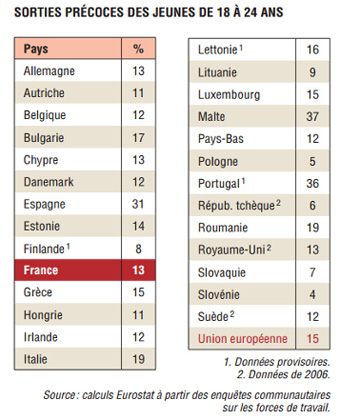
\includegraphics[scale=0.5]{stat12.jpg} 
\end{minipage}

\begin{enumerate}
\item Détermine la médiane des sorties précoces en Europe. 

\item 
\begin{enumerate}
\item Compléter le tableau suivant.

\begin{tabular}{|c|c|c|c|c|c|c|}
\hline 
Sorties précoces en 2007 & [0;5[ & [5;10[ & [10;15[ & [15;20[ & [20;25[ & [25;30] \\ 
\hline 
Effectif de pays européens &  &  &  &  &  &  \\ 
\hline 
E.C.C. des pays européens &  &  &  &  &  &  \\ 
\hline 
\end{tabular} 

\item Construis le polygone des effectifs cumulés croissants.

\item En déduire la médiane des sorties précoces en Europe. 
 
\item Compare avec la question 1.
\end{enumerate}
\end{enumerate}



  
\end{AD}

\begin{DefT}{Etendue}
On appelle \textbf{étendue} d'une série statistique la différence entre la plus grande valeur de la série et la plus petite valeur de la série.
\end{DefT}



\begin{AD}

Lors du devoir commun de Quatrième, voici les résultats de 2 classes.

\begin{minipage}{0.5\linewidth}
\begin{center}
\textbf{Quatrième  1}


\begin{tabular}{|c|c|c|c|c|c|}
\hline 
20 & 18 & 25 & 28& 35 & 27 \\ 
\hline 
22 & 17 & 15 & 26 &37 & 30 \\ 
\hline 
12 & 20 & 21 & 21 & 22 & 30 \\ 
\hline 
30 & 33 & 32 & 23 & 22 & 32 \\ 
\hline 
\end{tabular} 
\end{center}
\end{minipage}
\begin{minipage}{0.5\linewidth}
\begin{center}
\textbf{Quatrième  2}


\begin{tabular}{|c|c|c|c|c|c|}
\hline 
21 & 15 & 25 & 28& 35 & 27 \\ 
\hline 
39 & 9 & 15 & 26 &37 & 30 \\ 
\hline 
15 & 20 & 22 & 21 & 22 & 35 \\ 
\hline 
30 & 30 & 32 & 27 & 29 & 33 \\ 
\hline 
\end{tabular} 
\end{center}
\end{minipage}

\begin{enumerate}
\item Calculer l'étendue de chaque classe.
\item Quelle est la classe la plus hétérogène ?
\item Calculer la médiane de chaque classe.
\item Interpréter les résultats statistiques.
\end{enumerate}
\end{AD}





\begin{autoeval}
\begin{tabular}{p{12cm}p{0.5cm}p{0.5cm}p{0.5cm}p{1cm}}
\textbf{Compétences visées} &  M I & MF & MF  & TBM \vcomp \\ 
Calculer une médiane & $\square$ & $\square$  & $\square$ & $\square$ \\ 
Calculer une étendue & $\square$ & $\square$ & $\square$ & $\square$  \\ 
Interpréter une caractéristique de position& $\square$ & $\square$  & $\square$ & $\square$ \\ 
Interpréter une caractéristique de dispersion & $\square$ & $\square$ & $\square$ & $\square$ \\ 
\end{tabular}
{\footnotesize MI : maitrise insuffisante ; MF = Maitrise fragile ; MS = Maitrise satisfaisante ; TBM = Très bonne maitrise}
 
\end{autoeval} % Calculer une médiane, une étendue



\end{document}